En la figura \ref{fig:diagramacalibracion} se muestra un diagrama de flujo que resume el proceso de calibración que se desarrolla en el programa.\\
\begin{figure}[H]
	\centering
	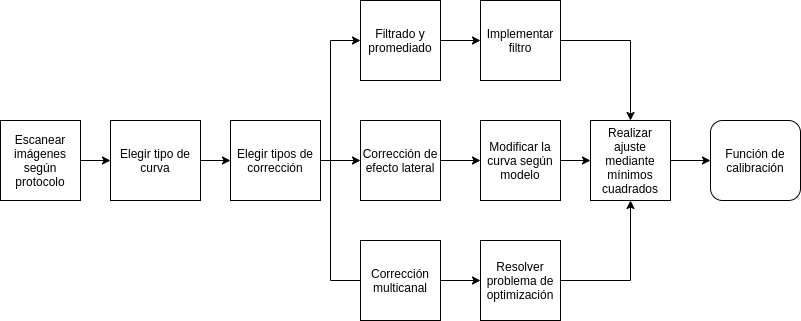
\includegraphics[width=\linewidth]{images/daigramaFlujo.png}
	\caption{Diagrama de flujo para calibración }
	\label{fig:diagramacalibracion}
\end{figure}
Análogamente, en la figura \ref{fig:diagramaMapa} se muestra un diagrama de flujo del proceso de construcción de un mapa de dosis.\\
\begin{figure}[H]
	\centering
	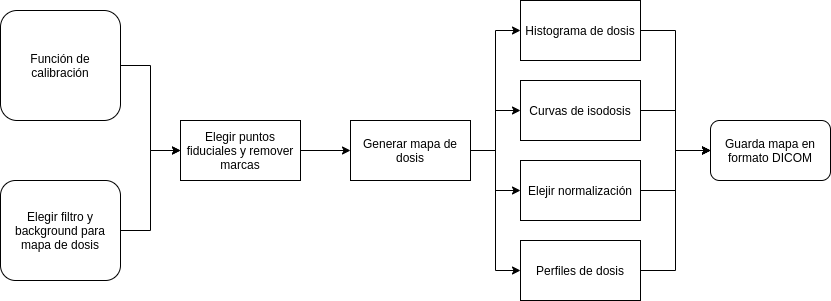
\includegraphics[width=\linewidth]{images/daigramaMapaDosis2.png}
	\caption{Diagrama de flujo para generación de mapa de dosis }
	\label{fig:diagramaMapa}
\end{figure}
Finalmente, en la figura \ref{fig:diagramaComparacion} se muestra un diagrama del proceso de comparación entre un plan calculado por el sistema de planeación y un mapa de dosis obtenido mediante una película radiocrómica.
\begin{figure}[H]
	\centering
	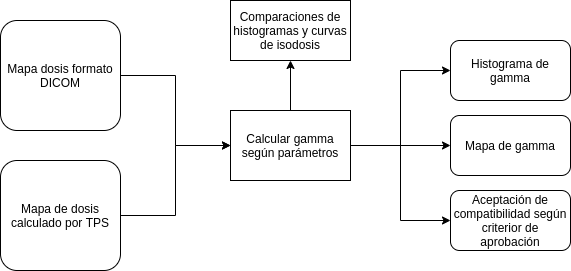
\includegraphics[width=\linewidth]{diagramaComparacion.png}
	\caption{Diagrama de flujo para comparación plan-mapa }
	\label{fig:diagramaComparacion}
\end{figure}